\documentclass{scrartcl}[a4paper,10pt,headings=small,footinclude=false]
\usepackage[bottom=3cm,top=3cm,
  %,showframe% <- only to show the page layout
]{geometry}
\setkomafont{disposition}{\normalfont\bfseries}
%\setkomafont{section}{\normalfont\normalsize\bfseries}
\setlength{\parskip}{.5em}
\usepackage[french]{babel}
%\usepackage[default]{fontsetup}


\usepackage[
  activate={true,nocompatibility},
  final,
  tracking=true,
  factor=1200,
  stretch=50,
  shrink=0
  ]{microtype}

%\usepackage{stix2}
\usepackage{hyperref}
\usepackage{fontspec}
\usepackage{unicode-math}
%\setmathfont{STIX Two Math}
%\setmainfont{STIX Two Text}
%\setmainfont{Latin Modern Roman}
%\setmathfont{Latin Modern Math}
\usepackage[default]{fontsetup}
\usepackage{amsfonts,amsmath,amsthm,stmaryrd,bm}
\usepackage[frenchkw,linesnumbered]{algorithm2e}
\usepackage{enumitem}

\theoremstyle{definition}
\newtheorem{theorem}{Théorème}[section]
\newtheorem{corollary}{Corollaire}[theorem]
\newtheorem{lemma}[theorem]{Lemme}
\newtheorem{proposition}[section]{Proposition}


\newtheorem{definition}{Définition}[section]
\theoremstyle{remark}
\newtheorem*{remark}{Remarque}
\newtheorem*{example}{Exemple}
\newtheorem*{exercise}{Exercice}
%\renewcommand{\qedsymbol}{$\vrectangle$}

\renewcommand{\qedsymbol}{}


\usepackage{graphicx}
\usepackage{float}

\title{Projets de codes correcteurs}
\author{\normalsize Julien Coolen}
\date{\normalsize\today}

\begin{document}
\maketitle
\tableofcontents

\section{Décodage par syndrôme}
\subsection{Algorithme de Prange}

\begin{algorithm}[H]
    \renewcommand{\algorithmcfname}{Algorithme}%
    \SetAlgoLined
    \Donnees{$\textbf{H}\in\mathbb{F}_q^{(n-k)\times n}$, $\textbf{s}\in\mathbb{F}_q^{n-k}$, $w\in\llbracket 0, n\rrbracket$.}
    \Res{$\textbf{e}\in\mathbb{F}_q^{n}$ tel que $\textbf{H}\textbf{e}^T = \textbf{s}$ et $|\textbf{e}|\leq w$.}
    \Repeter{$|\textbf{s}'| \leq w$}{
        Choisir $I\subseteq \llbracket 1,n\rrbracket$ tel que $|I|=k$ et $J=\llbracket 1,n\rrbracket \setminus I$

        \Si{$\textbf{H}_{J}$ est inversible}{
            $\textbf{s}'\leftarrow\textbf{H}_{J}^{-1}\textbf{s}^T$
        }
    }
    \Retour{$\textbf{e}$ tel que $\textbf{e}_I=\textbf{0}$ et $\textbf{e}_J = \textbf{s}'^T$.}
\caption{Algorithme de Prange (1962) (type Las Vegas)}
\end{algorithm}
\begin{proof}[Preuve de l'algorithme de Prange]
On a bien $|\textbf{e}|=\underbrace{|\textbf{e}_I|}_{= 0}+|\textbf{e}_J|\leq w$ car $I$ et $J$ sont disjoints.
De plus la sortie $\textbf{e}$ de l'algorithme vérifie bien
\begin{align*}
    \textbf{He}^T &= \textbf{H}(\textbf{e}_I+\textbf{e}_J)^T\\
    &= \textbf{H}_I \textbf{e}_I^T + \textbf{H}_J \textbf{e}_J^T\\
    &= \textbf{0} + \textbf{H}_J \textbf{H}_J^{-1} \textbf{s}\\
    &= \textbf{s}.
\end{align*}
\end{proof}


Soit un code linéaire $[n,k]_q$ et $w\in\llbracket 0, (1-\frac{1}{q})(n-k)\rrbracket$.
La complexité de Prange est

\[ T_{\text{Prange}} = O\Bigg(\frac{\min \big\{ \binom{n}{w}(q-1)^w, q^{n-k} \big\}}{\binom{n-k}{w}(q-1)^w}\Bigg). \]

\begin{proof}
La probabilité de succès d'une itération de l'algorithme est dans le pire cas ($|\textbf{e}|=w$):
\[ \mathbb{P}_{\text{succès}} \geq \frac{\binom{n-k}{w}(q-1)^w}{\binom{n}{w}(q-1)^w} \max \{1, |\text{DecSynd}(\textbf{H},\textbf{s},w)|\}\]

avec 
\[ |\text{DecSynd}(\textbf{H},\textbf{s},w)| = q^k \frac{\binom{n}{w}(q-1)^w}{q^n}. \]

D'où
\begin{align*}
    \mathbb{P}_{\text{succès}} &\geq \frac{\binom{n-k}{w}(q-1)^w}{\binom{n}{w}(q-1)^w} \max \Big\{1,\frac{\binom{n}{w}(q-1)^w}{q^{n-k}}\Big\}\\
    &\geq \binom{n-k}{w}(q-1)^w \max \Big\{\frac{1}{\binom{n}{w}(q-1)^w},\frac{1}{q^{n-k}}\Big\}\\
    &\geq \binom{n-k}{w}(q-1)^w \frac{1}{\min \{\binom{n}{w}(q-1)^w,q^{n-k}\}}.
\end{align*}
\end{proof}

Le coût $C$ d'une itération est dominé par le coût polynomial de l'élimination gaussienne sur $\mathbb{F}_q$: $C=n(n-k)^2\log^2 q$. En effet, on effectue $n(n-k)$ opérations sur les colonnes, et une multiplication sur $\mathbb{F}_q$ requiert $O(\log^2 q)$ opérations en bits.

Bien que le coût d'une itération est dominé par les facteurs exponentiels, on doit le garder dans le grand $O$ car c'est un facteur non constant (polynomial):
\begin{align*}
    T_{Prange} &= O\Big(C \cdot \frac{1}{\mathbb{P}_{\text{succès}}}\Big)\\
&= O\Bigg(\frac{n(n-k)^2(\log^2 q)\min \big\{\binom{n}{w}(q-1)^w,q^{n-k}\big\}}{\binom{n-k}{w}(q-1)^w} \Bigg).
\end{align*}

On pose $w=\lfloor \omega n \rfloor$.
La complexité asymptotique de Prange est $\tilde{O}(q^{n\alpha})$
avec \[\alpha\coloneq \min\big\{ h_q\big(\omega\big), 1-R \big\} - ( 1-R)h_q\bigg(\frac{\omega}{1-R}\bigg).\]

\begin{remark}
$T_{Prange}$ est maximal lorsque $\tbinom{n}{w}(q-1)^w=q^{n-k}$ donc lorsque $w=d_{GV}\coloneq h_q^{-1}(1-R)$. En effet $\delta_{GV}(R)\coloneq d_{GV}/n=h_q^{-1}(1-R)+o(1)$ et $\binom{n}{d_{GV}}(q-1)^{d_{GV}}=O(q^{nh_q(d_{GV}/n)})=O(q^{nh_q(h_q^{-1}(1-k/n))})=O(q^{n-k})$. %Mouais, pas super rigoureux le traitement du o(1)
\end{remark}

\begin{figure}[h]
\centering
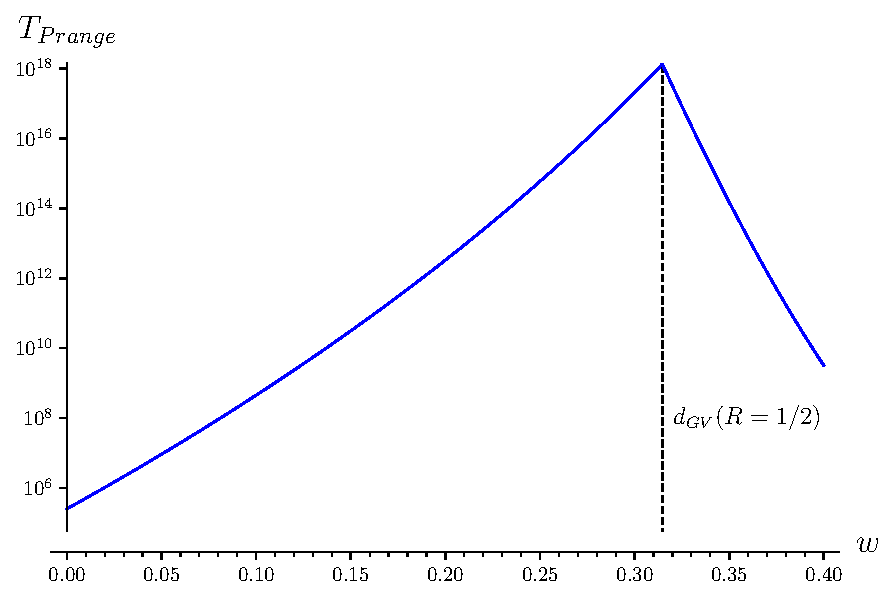
\includegraphics{decodage_syndrome/prange.pdf}
\caption{Complexité asymptotique de Prange pour un rendement $R=\frac{1}{2}$. $T_{Prange}$ est bien maximal pour la distance de Gilbert-Varshamov, la distance la plus difficile à décoder.}
\label{fig:prange}
\end{figure}


\subsection{Algorithme de Lee-Brickell}

L'idée est de relaxer la condition de Prange ($|\textbf{e}_I|=0$) pour amortir le coût de l'élimination gaussienne: on prend $p\geq 0$ petit et on l'on retourne un vecteur $\textbf{e}$ tel que $|\textbf{e}_I|=p$ et $|\textbf{e}_J|\leq w-p$. Si $p=0$ il s'agit exactement de l'algo de Prange.

\begin{algorithm}[H]
    \renewcommand{\algorithmcfname}{Algorithme}%
    \SetAlgoLined
    \Donnees{$\textbf{H}\in\mathbb{F}_q^{(n-k)\times n}$, $\textbf{s}\in\mathbb{F}_q^{n-k}$, $w\in\llbracket 0, n\rrbracket$.}
    \Res{$\textbf{e}\in\mathbb{F}_q^{n}$ tel que $\textbf{H}\textbf{e}^T = \textbf{s}$ et $|\textbf{e}|\leq w$.}
    \Repeter{$\exists \textbf{y}\in\mathcal{L}, |\textbf{y}|\leq w-p$}{
        Choisir un ensemble d'information $I\subseteq\llbracket 1,n\rrbracket$, $|I|=k$, et son complémentaire $J$
        
        \Si{$\textbf{H}_{J}$ est inversible}{
            $\mathcal{L}\leftarrow\{ \textbf{H}_J^{-1}\textbf{s} - \textbf{H}_J^{-1}\textbf{H}_I\textbf{x}^T : |\textbf{x}|=p\}$
        }
    }
    \Retour{$\textbf{e}$ tel que $\textbf{e}_I=\textbf{x}$ et $\textbf{e}_J = \textbf{y}^T$ ($\textbf{y}$ obtenu à partir de $\textbf{x}$, $\mathcal{L}$ est une table de hachage).}
\caption{Algorithme de Lee-Brickell}
\end{algorithm}

\begin{proof}[Preuve de l'algorithme de Lee-Brickell]
On a bien $|\textbf{e}|=|\textbf{e}_I|+|\textbf{e}_J|\leq p + (w - p)\leq w$ car $I$ et $J$ sont disjoints.
De plus la sortie $\textbf{e}$ de l'algorithme vérifie bien
\begin{align*}
    \textbf{He}^T &= \textbf{H}(\textbf{e}_I+\textbf{e}_J)^T\\
    &= \textbf{H}_I \textbf{x}^T + \textbf{H}_J \textbf{y}\\
    &= \textbf{H}_I \textbf{x}^T + \textbf{H}_J (\textbf{H}_J^{-1}\textbf{s} - \textbf{H}_J^{-1}\textbf{H}_I\textbf{x}^T)\\
    &= \textbf{s}.
\end{align*}
\end{proof}

Le coût d'une itération est dominé par l'énumération $C=n(n-k)^2(\log^2 q) + \binom{k}{p}(q-1)^p=O(\binom{k}{p}(q-1)^p)$ et non plus par le pivot de Gauss. 
%Pour un pattern d'erreur, on que $\mathcal{P}_\infty=\frac{\binom{n-k}{w-p}\binom{k}{p}}{\binom{n}{w}}$ et $\mathcal{N}_\infty = \frac{\binom{n}{w}}{\binom{n-k}{w-p}\binom{k}{p}}$ and $C=n^3 + \binom{k}{p}$.


% Faux! à recalculer, mais oui on gagne un facteur poly
La proba de succès est dans le pire cas ($|\textbf{e}|=w$):

\begin{align*}
\mathbb{P}_{\text{succès}} &\geq  \frac{\binom{n-k}{w-p}(q-1)^{w-p} \binom{k}{p}(q-1)^{p}}{\binom{n}{w}(q-1)^w} \max \{ 1, |\text{DecSynd}(\textbf{H},\textbf{s},w)|\}\\
&\geq  \frac{\binom{n-k}{w-p} \binom{k}{p}}{\binom{n}{w}} \max \{ 1, |\text{DecSynd}(\textbf{H},\textbf{s},w)|\}\\
&\geq  \frac{\binom{n-k}{w-p} \binom{k}{p}}{\binom{n}{w}} \max \{ 1, q^k \frac{\binom{n}{w}(q-1)^w}{q^n}\}\\
&\geq  \binom{n-k}{w-p} \binom{k}{p} \max \{ \frac{1}{\binom{n}{w}}, \frac{(q-1)^w}{q^{n-k}}\}\\
&\geq  \binom{n-k}{w-p} \binom{k}{p} \frac{1}{\min \{ \binom{n}{w}, \frac{q^{n-k}}{(q-1)^w}\}}\\
&\geq  \binom{n-k}{w-p} \binom{k}{p} \frac{(q-1)^w}{\min \{ \binom{n}{w}(q-1)^w, q^{n-k}\}}.
\end{align*}

On ne gagne jamais plus qu'un facteur polynomial sur Prange (le coût du pivot):
\begin{align*}
T_{LB} &= C\cdot \frac{1}{\mathbb{P}_{\text{succès}}}\\
&=\Bigg(n(n-k)^2(\log^2 q) + \binom{k}{p}(q-1)^p\Bigg)  \frac{\min \{ \binom{n}{w}(q-1)^w, q^{n-k}\}}{\binom{n-k}{w-p} \binom{k}{p}(q-1)^w}\\
&=\Bigg(\frac{n(n-k)^2(\log^2 q)}{\binom{k}{p}} +(q-1)^p\Bigg)  \frac{\min \{ \binom{n}{w}(q-1)^w, q^{n-k}\}}{\binom{n-k}{w-p} (q-1)^w}\\
&\geq \frac{\min \{ \binom{n}{w}(q-1)^w, q^{n-k}\}}{\binom{n-k}{w-p} (q-1)^w}\\
&\geq \frac{\min \{ \binom{n}{w}(q-1)^w, q^{n-k}\}}{\binom{n-k}{w} (q-1)^w}\\
&\geq \frac{1}{n(n-k)^2(\log^2 q)} T_{Prange}.
\end{align*}

La complexité de Lee-Brickell est donc (pivot dominé par l'énumération), pour $w=\lfloor \omega n \rfloor$ et $\rho=\lfloor \frac{p}{n} \rfloor$:

\[
	O\Bigg(\frac{\min \{ \binom{n}{w}(q-1)^w, q^{n-k}\}}{\binom{n-k}{w-p} (q-1)^{w-p}}\Bigg).
\]

La complexité asymptotique de Lee-Brickell est $\tilde{O}(q^{n\alpha})$ pour

\[
\alpha \coloneq \min\{ h_q(\omega), 1-R \} - (1-R) h_q\bigg(\frac{\omega - \rho}{1-R}\bigg).
\]

\begin{figure}[h]
\centering
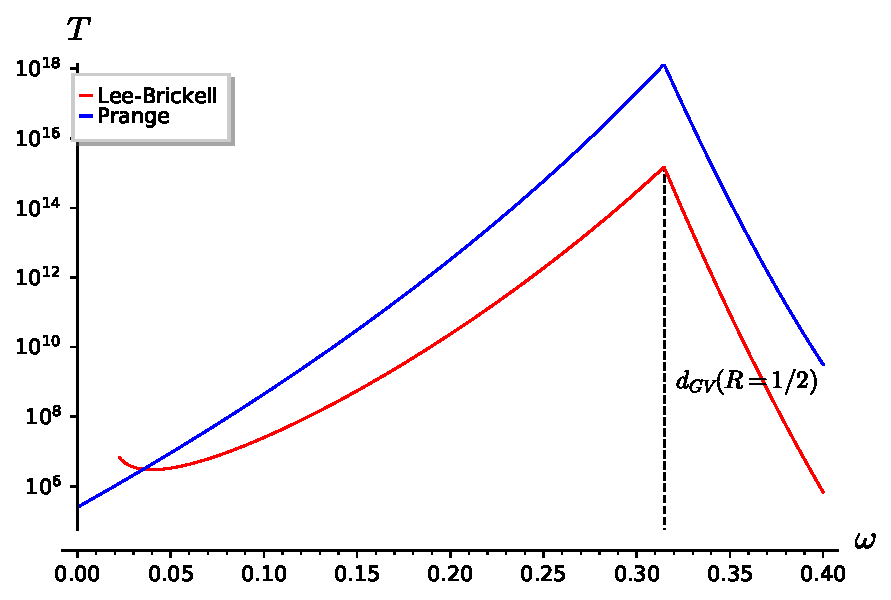
\includegraphics{decodage_syndrome/LB.pdf}
\caption{Complexité asymptotique de Lee-Brickell pour un rendement $R=\frac{1}{2}$ et $p=2$. La distance de Gilbert-Varshamov est la plus difficile à décoder. On observe bien le gain d'un facteur polynomial $O(n^3)$ avec l'échelle logarithmique: pour de petites valeurs de $w$ l'amélioration se dégrade.}
\label{fig:prange}
\end{figure}

Quelle est la valeur optimale de $p$ ?

On suppose que $R=\frac{1}{2}$ et $n$ très grand constant.
Étudions les variations de la fonction
\[
f(w)= \frac{1}{2} h_q\bigg(\frac{2(w - p)}{n}\bigg).
\]


Sauf pour $w$ très petit ou très grand, $p=2$ est optimal.



\subsection{Algorithme de Stern}

L'idée est de combiner Lee-Brickell et le décodage par paradoxe des anniversaires. On effectue une élimination gaussienne partielle.

Décodage par le paradoxe des anniversaires:
Problème: trouver au plus $w$ colonnes de $\textbf{H}$ dont la somme vaut $\textbf{s}$ sur $\mathbb{F}_q$.

Solution: scinder $\textbf{H}$ en deux parties égales et énumérer les deux ensembles
\[\mathcal{L}_1=\big\{ \textbf{s}-\textbf{H}_1\textbf{e}_1^T : wt(\textbf{e}_1) =\frac{w}{2} \big\}\]
et \[\mathcal{L}_2=\big\{ \textbf{H}_2 \textbf{e}_2^T : wt(\textbf{e}_2) = \frac{w}{2}\big\}.\]
Si $\mathcal{L}_1\cap \mathcal{L}_2\neq \emptyset$, on a des solutions $\textbf{s}-\textbf{H}\textbf{e}_1^T-\textbf{H}_2\textbf{e}_2^T=\textbf{0}$.

\begin{algorithm}[H]
    \renewcommand{\algorithmcfname}{Algorithme}%
    \SetAlgoLined
    \Donnees{$\textbf{H}\in\mathbb{F}_q^{(n-k)\times n}$, $\textbf{s}\in\mathbb{F}_q^{n-k}$, $w\in\llbracket 0, n\rrbracket$.}
    \Res{$\textbf{e}_\in\mathbb{F}_q^{n}$ tel que $\textbf{H}\textbf{e}^T = \textbf{s}$ et $|\textbf{e}|\leq w$.}
    $X=\{ \textbf{x}\in\mathbb{F}_q^{k/2} :|\textbf{x}| =\frac{p}{2} \}$
    
    \Repeter{$\exists (\textbf{x}_1, \textbf{y}), (\textbf{x}_2, \textbf{y}) \in\mathcal{L}_1 \cap \mathcal{L}_2, |\textbf{y}_{\llbracket 1,n \rrbracket \setminus L}|\leq w-p$}{
        Choisir un ensemble d'information $I\subseteq\llbracket 1,n\rrbracket$, $|I|=k$, et son complémentaire $J$
        
        \Si{$\textbf{H}_{J}$ est inversible}{
        
        		$\bar{\textbf{s}} \leftarrow \textbf{H}_J^{-1} \textbf{s}$
        		
        		$\bar{\textbf{A}}\leftarrow \textbf{H}_J^{-1} \textbf{H}_I$
        	
        		On extrait les deux sous-matrices $\bar{\textbf{A}}=[\bar{\textbf{A}}_1 \bar{\textbf{A}}_2 ]$
        		
            $\mathcal{L}_1\leftarrow \big\{  (\textbf{x}, \bar{\textbf{s}}-\bar{\textbf{A}}_1 \textbf{x}^T) : \textbf{x}\in X \big\}$
            
        			
            $\mathcal{L}_2\leftarrow\big\{ (\textbf{x},\bar{\textbf{A}}_2 \textbf{x}^T) : \textbf{x}\in X \big\}$
            
            Choisir un ensemble $L$ de $l$ positions
        }
    }
    \Retour{$\textbf{e}$ tel que $\textbf{e}_I=\textbf{x}$ et $\textbf{e}_J = \textbf{y}^T$ ($\textbf{y}$ obtenu à partir de $\textbf{x}$, $\mathcal{L}$ est une table de hachage).}
\caption{Algorithme de Stern}
\end{algorithm}

L'algorithme est correct, et la preuve est analogue à celle de Lee-Brickell (même calcul avec $\textbf{e}_I=\textbf{x}_1+\textbf{x}_2$).

On se place dans le pire des cas ($|\textbf{e}|=w$).
Une solution est trouvée à la fin d'une itération si $\textbf{e}_i$ est de poids $p$ (événement $E_1$), que de plus le poids de $\textbf{e}_i$ soit distribué de manière égale en $\textbf{x}_1$ et $\textbf{x}_2$ (événement $E_2$), et enfin que $l$ positions de $\textbf{e}_j$ de poids $w-p$ soient nulles (événement $E_3$).

On obtient, les événements étant indépendants:

\begin{align*}
\mathbb{P}_{\text{succès}} &\geq P(E_1 \wedge E_2 \wedge E_3)\\
&\geq \mathbb{P}(E_1) \mathbb{P}(E_2) \mathbb{P}(E_3)\\
&\geq \frac{\binom{k}{p}\binom{n-k}{w-p}}{\binom{n}{w}} \frac{\binom{k/2}{p/2}^2}{\binom{k}{p}} \frac{\binom{n-k-(w-p)}{l}}{\binom{n-k}{l}} \quad \text{car les puissances de } (q-1) \text{ se simplifient}\\
&\geq \frac{\binom{k/2}{p/2}^2\binom{n-k-l}{w-p}}{\binom{n}{w}} \quad \text{car } \frac{\binom{n-k}{w-p}\binom{n-k-(w-p)}{l}}{\binom{n-k}{l}} = \binom{n-k-l}{w-p} \text{ en explicitant les factorielles}.
\end{align*}

Le coût d'une itération est dominé par la recherche de collision et les multiplications de matrices: $C=\binom{k/2}{p/2}(q-1)^{p/2}(k/2)^3$.

On obtient donc comme complexité temporelle

\begin{align*}
	T_{Stern} &= C \cdot \frac{1}{P_{Stern}}\\
	&= \binom{k/2}{p/2}(q-1)^{p/2}(k/2)^3 \frac{\binom{n}{w}(q-1)^w}{\binom{k/2}{p/2}^2 (q-1)^p \binom{n-k-l}{w-p}(q-1)^{w-p}}\\
	&= O\Big(k^3 \frac{\binom{n}{w}(q-1)^w}{\binom{k/2}{p/2} (q-1)^{p/2} \binom{n-k-l}{w-p}(q-1)^{w-p}}\Big).
\end{align*}

Sa complexité asymptotique est, pour $w=\lfloor \omega n \rfloor, p = \lfloor \rho n \rfloor, l= \lfloor \lambda  n \rfloor$, $\tilde{O}(q^{n\alpha})$ avec

\[
	\alpha \coloneq h_q(\omega)-\frac{R}{2} h_q(\frac{\rho}{R}) - (1-R-\lambda)h_q(\frac{\omega - \rho}{1 - R - \lambda}).
\]

\begin{figure}[h!]
\centering
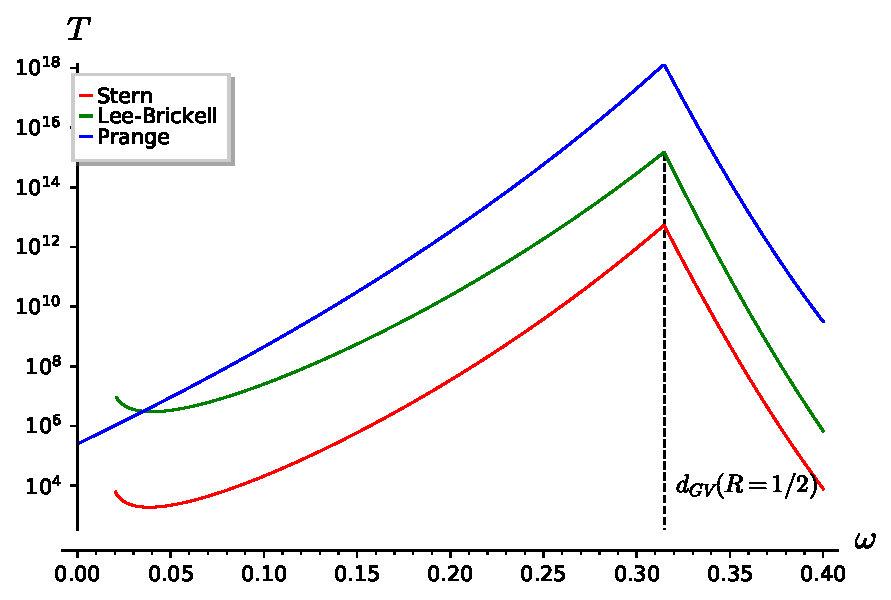
\includegraphics{decodage_syndrome/Stern.pdf}
\caption{Complexité asymptotique de Stern pour un rendement $R=\frac{1}{2}$.}
\label{fig:prange}
\end{figure}


\newpage
\section{Décodage en liste}


\end{document}
